% Figure 1.1 (Session 1): the dimension of the single-particle and of the many-body problem.
% The image is rendered by figures/blender/s1_1_exponential_wall.py; the coordinates of the labels
% come from figures/blender/out/exponential_wall_anchors.tex. Compile with:
%   pdflatex exponential_wall.tex ; result moves to ../classical_magnetism/exponential_wall.pdf
\documentclass[11pt,tikz,border=0pt]{standalone}
\usepackage{amsmath,amssymb,graphicx}
\usepackage{xcolor}
\definecolor{coursedark}{HTML}{1B2A4A}
\definecolor{costamber}{HTML}{B8620A}
\newlength{\figw}\setlength{\figw}{16.19cm}   % the text width of the notes (letter, 2.7 cm margins), so labels print at size

\begin{document}
\begin{tikzpicture}[lbl/.style={font=\small, text=coursedark}]
  \node[anchor=south west, inner sep=0pt] at (0,0)
    {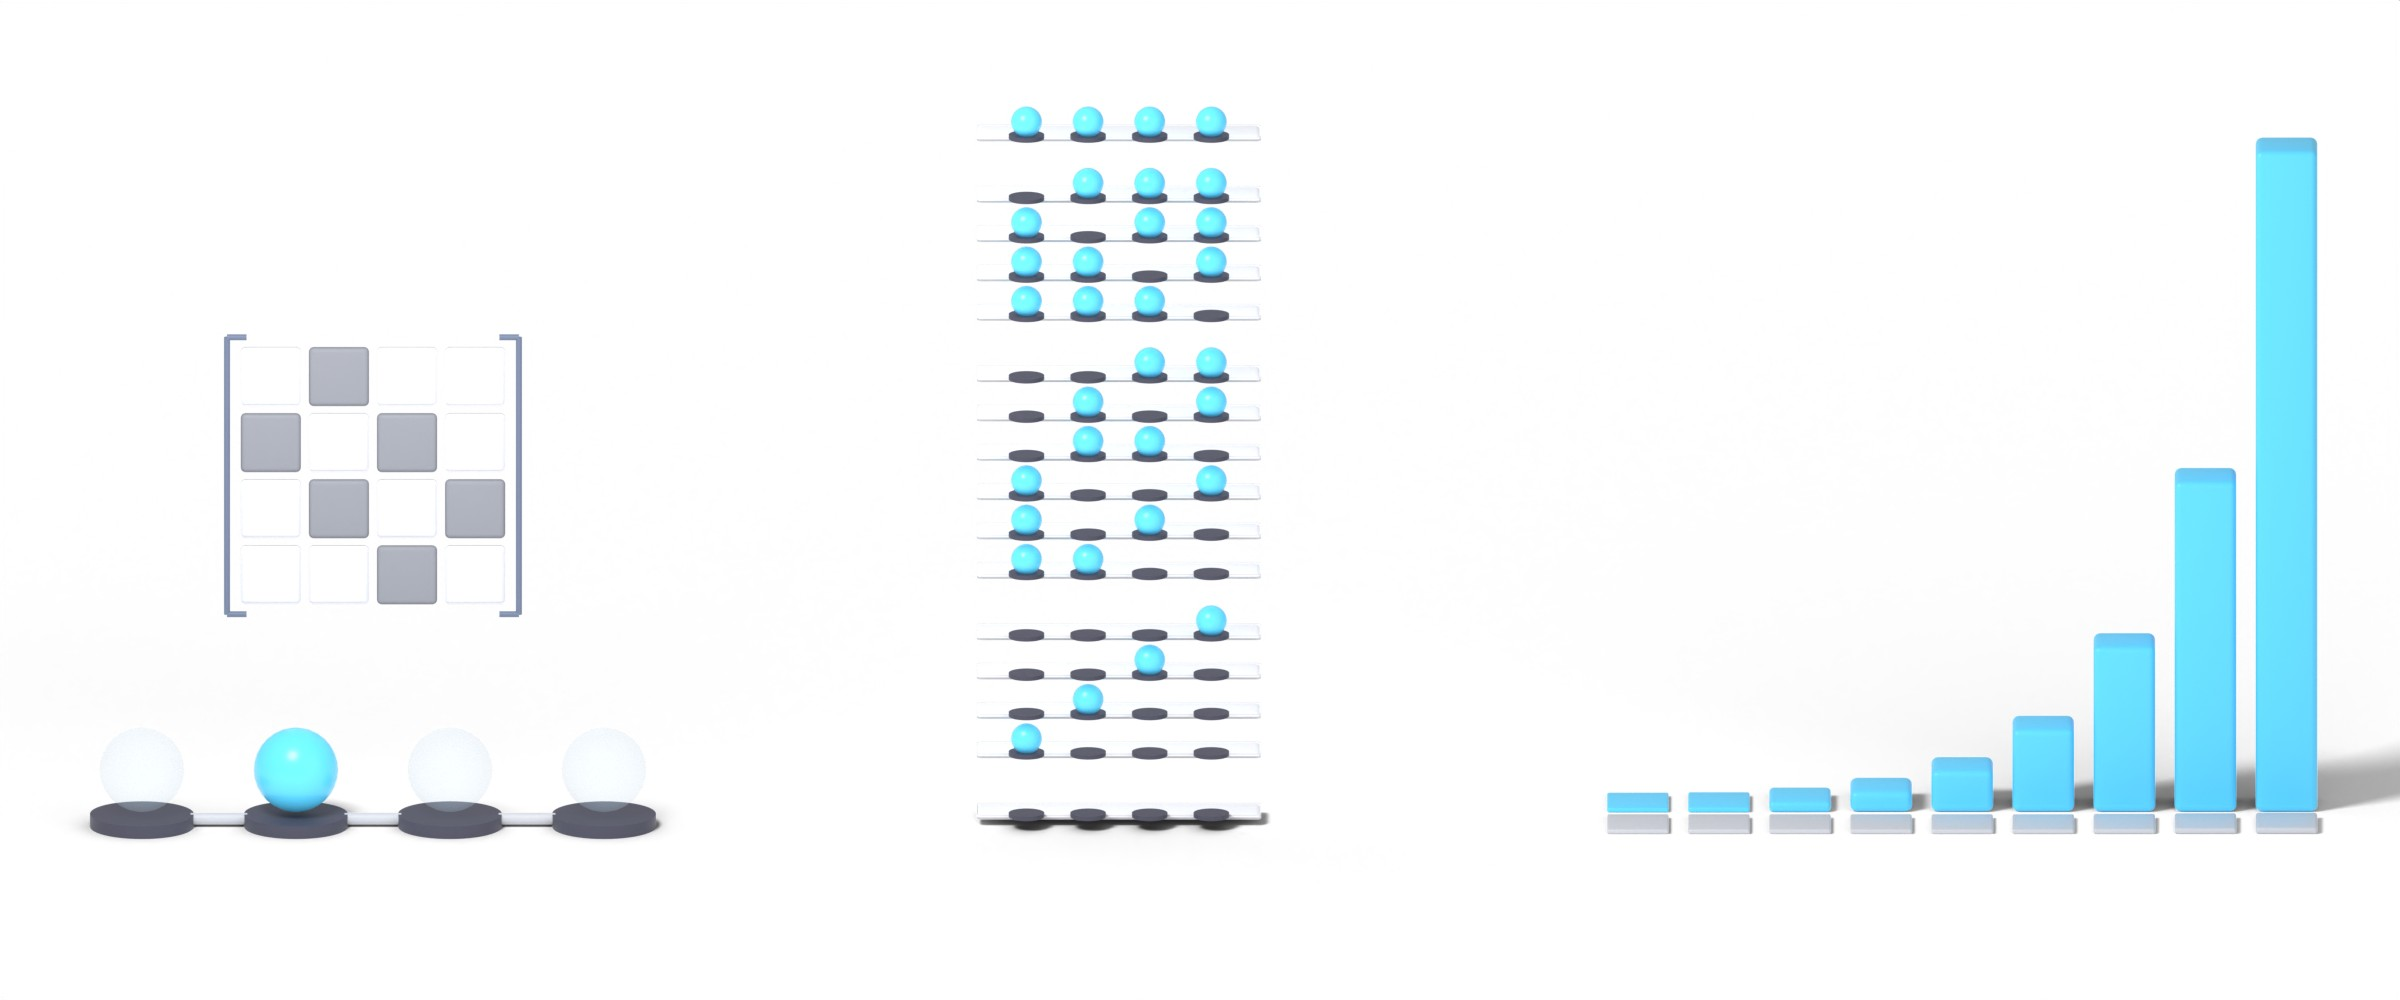
\includegraphics[width=\figw]{../blender/out/exponential_wall.jpg}};
  %% written by figlib.py; x and y in units of the image width
\coordinate (matA) at (0.2155\figw,0.2184\figw);
\coordinate (a) at (0.0203\figw,0.3739\figw);
\coordinate (countA) at (0.1554\figw,0.0576\figw);
\coordinate (N0) at (0.5321\figw,0.0802\figw);
\coordinate (N1) at (0.5321\figw,0.1303\figw);
\coordinate (N2) at (0.5321\figw,0.2215\figw);
\coordinate (N3) at (0.5321\figw,0.3126\figw);
\coordinate (N4) at (0.5321\figw,0.3627\figw);
\coordinate (b) at (0.3581\figw,0.3739\figw);
\coordinate (countB) at (0.4662\figw,0.0576\figw);
\coordinate (L2) at (0.6824\figw,0.0666\figw);
\coordinate (L6) at (0.8176\figw,0.0666\figw);
\coordinate (L10) at (0.9527\figw,0.0666\figw);
\coordinate (top) at (0.9358\figw,0.3599\figw);
\coordinate (mb) at (0.8682\figw,0.2121\figw);
\coordinate (sp) at (0.6622\figw,0.0723\figw);
\coordinate (c) at (0.6419\figw,0.3739\figw);

  \node[lbl, font=\normalsize, anchor=west] at (a) {(a)};
  \node[lbl, font=\normalsize, anchor=west] at (b) {(b)};
  \node[lbl, font=\normalsize, anchor=west] at (c) {(c)};
  \node[lbl, anchor=west] at (matA) {$t_{ij}$, $4\times4$};
  \node[lbl, anchor=north] at (countA) {4 states};
  \foreach \n/\d in {0/1,1/4,2/6,3/4,4/1} {
    \node[lbl, font=\footnotesize, anchor=west] at (N\n) {$N=\n$};
  }
  \node[lbl, anchor=north] at (countB) {$2^4=16$ states};
  \node[lbl, anchor=north] at (L2) {$2$};
  \node[lbl, anchor=north] at (L6) {$6$};
  \node[lbl, anchor=north] at (L10) {$10$};
  \node[lbl, anchor=south east] at (top) {$2^{10}=1024$};
  \node[lbl, anchor=east] at (mb) {$2^L$};
  \node[lbl, anchor=east] at (sp) {$L$};
\end{tikzpicture}
\end{document}
